\section{Methodology}
\label{sec:method}

An overview of the model architecture is shown in Figure \ref{fig:4}. Under the assumption that the two documents have comparable order in sentences, the model aligns the two texts as follows.
\begin{enumerate}
	\item Given a similarity measure $f_1$, the similarity measurement model computes the scores for all possible one-to-one pairs within a certain distance. This distance is defined as \texttt{MAX\_DISTANCE}, and is the maximum relative distance (given by the index of a sentence in the document) between two single sentences that are considered at this stage.
	\item Pairs whose similarity scores are above a given threshold $t$ are supposed to be the ``anchors'' and are appended to an anchor list. The anchors divide the original document into parts that are relatively shorter and easier for later alignment.
	\item For each part between two pairs of anchors, a local alignment algorithm is performed using a certain similarity measure, where we need to group the sentences and then align the groups. 
	\item Finally, an optional filtering process is performed. This is due to the observation that, including only one kind of similarity measure might result in unreasonable alignment or too strict alignment rules. To capture the semantic features in different perspectives, an additional similarity measure can be used to perform a filtering stage for sentences that are not successfully aligned at previous stages. At this stage, we only consider one-to-one alignment.
\end{enumerate}

\begin{figure}[htbp]
	\centering
	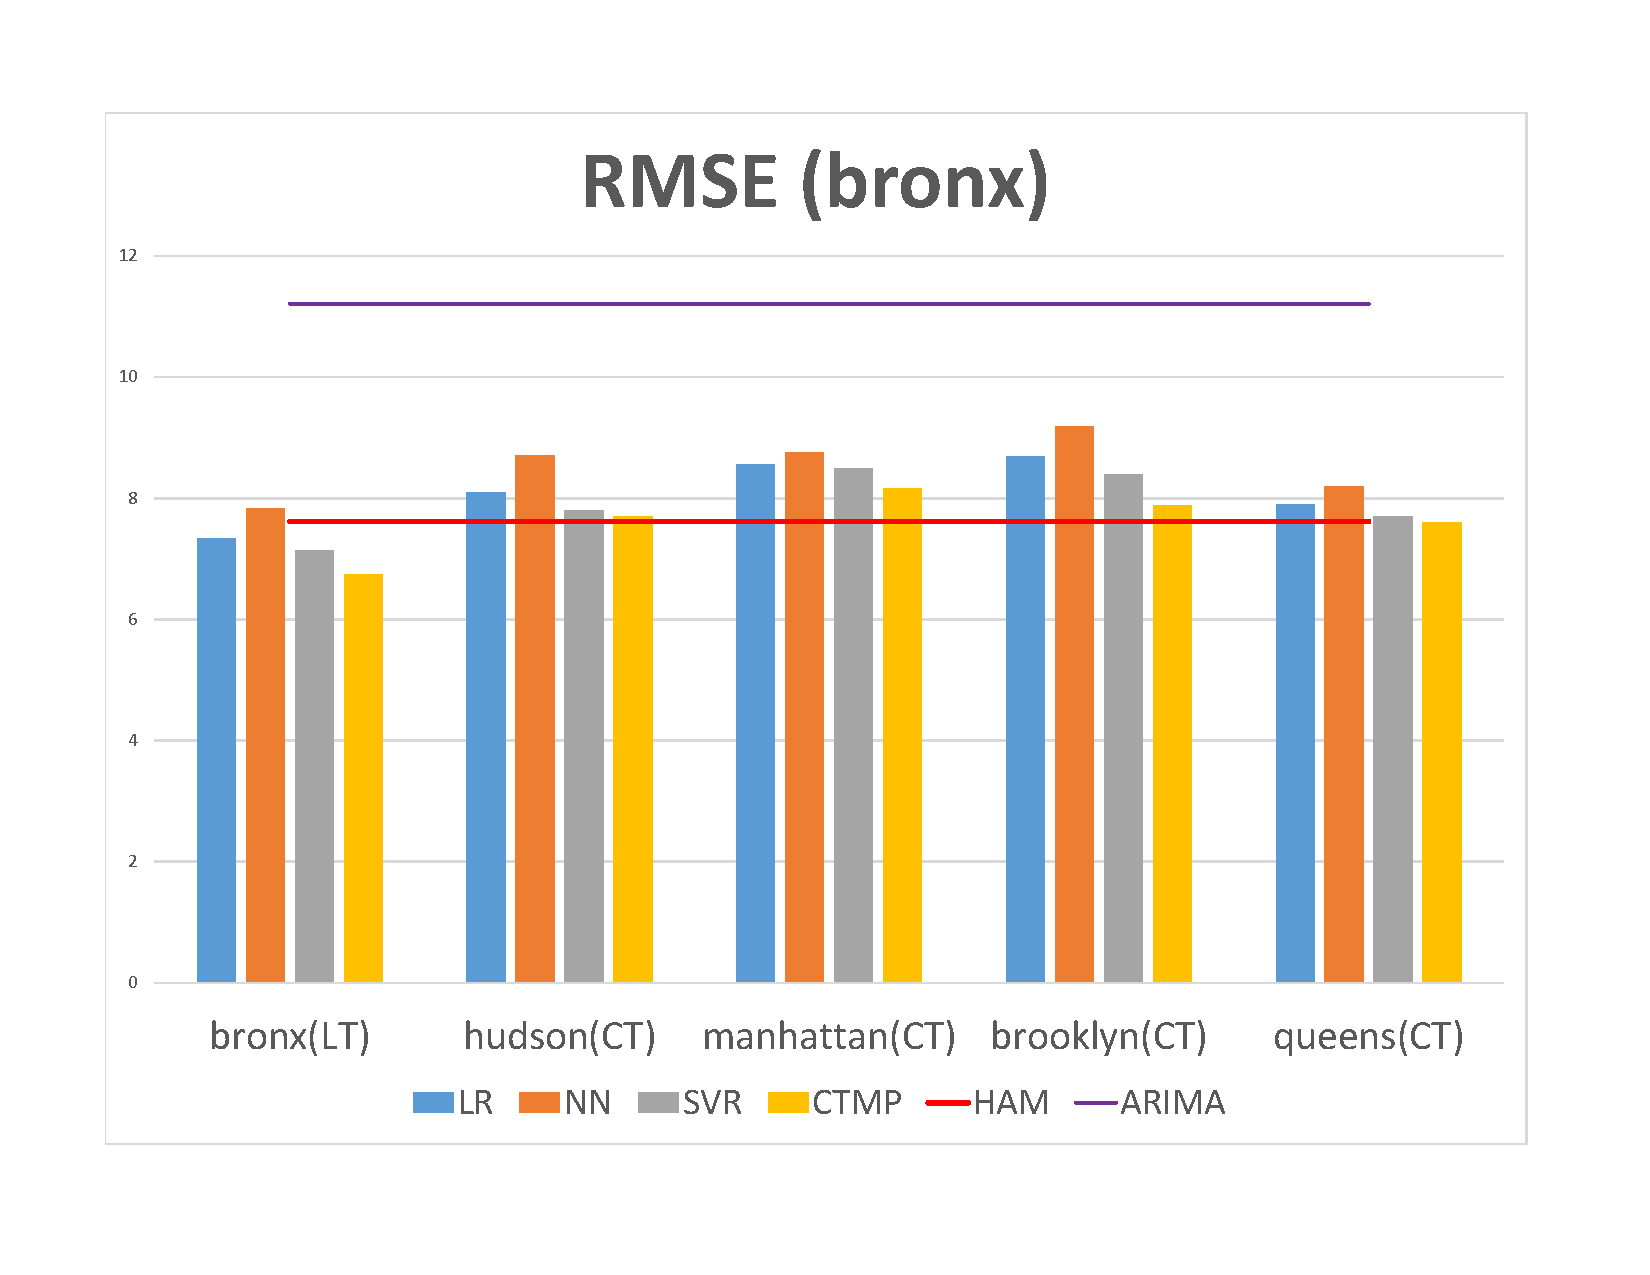
\includegraphics[width=8cm]{./4.png}
	\caption{Model Overview.}\label{fig:4}
\end{figure}

In sum, the model consists of basic similarity measurements and a local sequential alignment in each part separated by successive anchors. The effect of the final filtering stage will also be explored in this work.


\subsection{Similarity Measure}

The first subtask is to give a similarity score for each pair of sentences in order to further align them. In practice, the scoring requires a clustering strategy, since one-to-one sentence mapping is not necessarily required in the sequential alignment task. At this stage, we restrict ourselves to first evaluating the performance of different similarity measures. Namely, given two sentences $(w_1^{(a)}, w_2^{(a)}, \ldots, w_{l_a}^{(a)})$ and $(w_1^{(b)}, w_2^{(b)}, \ldots, w_{l_b}^{(b)})$, where each word in the sequence is a fixed dimensional vector $w_i^{(a)}, w_j^{(b)}\in \mathbb{R}^d$. Then each pair of the sentences $a, b$ are mapped to a score $r\in [0, 1]$ representing their sentence similarity. The compared models are evaluated based on their accuracies of paraphrase detection task, with corpora including MSRC, SICK, and Shakespeare scripts.

The general approach for unsupervised similarity measure is composed of a (hopefully strong) sentence representation model and a simple distance measure.
\begin{itemize}
	\item \textbf{Gensim Word2Vec (WDV).} The Gensim implementation of Word2Vec model uses CBOW and Skip-gram models~\cite{mikolov2013distributed}. In our implementation, the word vectors are trained on the two documents to be aligned, rather than using pretrained word vectors given by independent large corpus. This is under the consideration that, since our sentence alignment task is performed on stylized sentences, a corpus-specific Word2Vec model better fits in our scheme. 
	
	After obtaining word embeddings, the sentence embedding is the average of the sum of word vectors in a sentence. Then the final similarity is the average of word similarities according to a max alignment. Each word in sentence 1 is aligned to the most similar word in sentence 2, while each word in sentence 2 is aligned to the most similar word in sentence 1. Then the scores for the alignments in both directions are added and normalized by sentence length.
	\item \textbf{Universal Sentence Encoder (UNV).} Universal Sentence Encoder proposed by Cer et al.~\cite{cer2018universal} is designed to encode sentences into embedding vectors that specifically target transfer learning. This model is found to be useful in the filtering stage in this study.
	\item \textbf{InferSent Model (INF).} InferSent model first proposed as a Facebook research project of learning universal representations of sentences~\cite{conneau2017supervised}. In our study, we explore both GloVe and FastText pretrained word vectors proposed in their model~\cite{pennington2014glove, joulin2017bag}.
\end{itemize}

Using sentence embeddings, cosine and arccos measures are used to calculate the final similarity score, defined as follows.
\begin{align*}
sim_{\cos} & = \cos(v_1, v_2), \\
sim_{\arccos} & = \frac{\arccos(\cos(v_1, v_2))}{\pi}.
\end{align*}
Particularly, it is shown from the results that cosine distance measure is superior to the arccos measure.

These unsupervised methods are compared with the state-of-art supervised methods in paraphrase detection task, in order to evaluate the ability of the similarity measures used in the alignment. These methods include:
\begin{itemize}
	\item Siamese Recurrent Neural Networks (MaLSTM)~\cite{mueller2016siamese}.
	\item TF-KLD: a discriminative improvement to distributional sentence similarity proposed by Ji et al.~\cite{ji2013discriminative}.
\end{itemize}

\subsection{Sequential Alignment}

In our scheme of constructing parallel corpus from comparable documents, we need to consider (a) the documents being aligned are potentially large, and (b) there exist sentences that are aligned with two or more sentences from the other document, and there also exist sentences that are not aligned at all.

These two scenarios lead to challenges in designing the sequential alignment algorithm, since the grouping of the sentences are not known in advance, the similarity score for each pair of groups is not pre-calculated. Furthermore, exhaustive enumeration of all possible groupings is intractable. Therefore, we make the following assumptions.
\begin{enumerate}
	\item The number of sentences in each group does not exceed a maximum window size \texttt{MAX\_WINDOW\_SIZE} for each part enclosed by any two successive anchors of the document. Moreover, to handle the situation of shorter parts, the maximum number of sentences is proportional to a factor, defined as \texttt{SIZE\_PER\_TEN}. The scaled limit 
	$$w_{max} = \texttt{SIZE\_PER\_TEN} \times \texttt{len}(part) / 10$$
	is then compared with \texttt{MAX\_WINDOW\_SIZE}, and the minimum of them is the maximum number of sentences in a group. 
	\item Two aligned groups cannot appear farther than a limit \texttt{MAX\_DISTANCE}. The assumption is that the aligned groups in the two documents do not locate far from each other, considering relative distance for the whole document. Suppose the index of a sentence in \emph{doc1} is $i$, then the relative corresponding index in \emph{doc2} is defined by $j = i\cdot \dfrac{l_2}{l_1}$, where $l_k, k = 1, 2$ denotes the document length, and the sentences in \emph{doc2} out of the range [$j$ - \texttt{MAX\_LENGTH}, $j$ + \texttt{MAX\_LENGTH}] will not be considered.
\end{enumerate}

Based on these assumptions, we use a greedy alignment scheme. Between each successive pairs of anchors, the similarity scores for all possible pairs are calculated and sorted in decreasing order. In each pairing, the most similar pair is popped from the candidate list, and the remaining groups that include any sentence in the selected pair is deleted from the candidate list. The pairing stops until the similarity score for the most similar pair is below a predefined threshold, or the candidate list becomes empty. The greedy alignment process is illustrated in Algorithm \ref{alg:1}.

\begin{algorithm}
	\caption{Greedy Alignment.}
	\label{alg:1}
	\KwIn{A sorted array (based on similarity score $sim$) of sentence group pairs $Arr = [[g_1, g_2, sim], \ldots]$}
	\KwOut{An collection of paired sentence groups}
	$A\leftarrow \emptyset$\;
	\While{$Arr[0].sim > threshold$}{
		$p\leftarrow Arr.pop(0)$\;
		Add $p$ into $A$;
		\ForEach{sentence $s$ in $p.g_1$}{
			remove $p'$ from $Arr$ if $p'.g_1$ contains $s$\;
		}
		\ForEach{sentence $s$ in $p.g_2$}{
			remove $p'$ from $Arr$ if $p'.g_2$ contains $s$\;
		}
	}
	\textbf{return} $A$\;
\end{algorithm}
